\documentclass{modeleRapport}

\addbibresource{biblio.bib}
\usepackage{lmodern}
\hbadness=10000
\vbadness=10000
\scrollmode % Send warning to logs not to show them upon compiling

%--------------------------------------

\titre{AI Algorithms Project}
\soustitre{A biscuit problem}

\enseignant{Farah \textsc{AIT SALAHT} \\
}

\eleves{Hugo \textsc{BONNELL} \\
}

%--------------------------------------

\begin{document}

\fairepagedegarde
\fairetabledesmatieres

%--------------------------------------

\section{Problem Overview}

\subsection{The Problem}

\subsubsection{A biscuit factory}

A biscuit manufacturing factory is planning to produce a series of biscuits for Christmas. Using the same roll of dough, 
the factory aims to create various biscuits of different sizes and shapes. The goal is to maximize biscuit production from a 
single roll while ensuring the highest possible profit.

To achieve this goal, we have the following information :

\begin{itemize}
    \item The roll of dough has a predefined rectangular length, referred to as ’LENGTH’, representing a one-dimensional problem.
    
    \item The roll may contain irregularities, referred to as defects. Each defect has :
    \begin{itemize}
        \item a position ‘x‘
        \item and a class, which could be one of several types (e.g., ’a’, ’b’, ’c’, ...).
    \end{itemize}

    \item The factory aims to produce a set of biscuits. Each Biscuit can be produced an infinite number of times, and has :
    \begin{itemize}
        \item a specific size (along the same dimension as the roll)
        \item a value (price)
        \item and a threshold for the maximum number of defects of each class it can contain (otherwise it cannot be marketed).
    \end{itemize}
\end{itemize}

A solution is defined as an arrangement of biscuits along the dough roll. For an arrangement (assignment) to be valid, 
it must satisfy the following conditions :

\begin{itemize}
    \item Biscuits must be placed at integer positions.
    \item No overlapping of biscuits is allowed. For example, if you place a biscuit B1 of size 3 at position ‘x=2‘, no other 
    biscuit can be assigned to positions ‘x=3‘ or ‘x=4‘.
    \item Each biscuit placed must contain fewer defects (or an equal number) of each class than its permitted thresholds. 
    For instance, if biscuit B1 of size 3 is placed at ‘x=2‘, it covers positions 2, 3 and 4. If there are 3 defects of 
    class ’a’ in these positions, but B1’s threshold for class ’a’ is a maximum of 2 defects, then the assignment is invalid.
    \item The total size of the assigned biscuits must not exceed the length of the dough roll.
\end{itemize}

The value of a solution is the sum of the individual values of the biscuits placed on the roll. However, any portion of 
the dough roll without an assigned biscuit incurs a penalty of 1 per position, reflecting the company’s loss from wasted 
material. This penalty is subtracted from the overall value of the solution.

\newpage

\subsubsection{Benchmark}

For this project, the following assumptions are made :

\begin{itemize}
    \item The length of the roll of dough is set to \textbf{500 units.}
    \item The roll has three classes of defects (’a’, ’b’, and ’c’). The set of defects and their positions on the roll 
    are available in the ’defects.csv’ file.
    \item The biscuit manufacturing factory aims to produce 4 types of biscuits :
    \begin{itemize}
        \item Biscuit 0 with a length of 4, a value of 3, and maximum allowed defects as {'a' : 4, 'b' : 2, 'c' : 3}
        \item Biscuit 1 with a length of 8, a value of 12, and maximum allowed defects as {'a' : 5, 'b' : 4, 'c' : 4}
        \item Biscuit 2 with a length of 2, a value of 1, and maximum allowed defects as {'a' : 1, 'b' : 2, 'c' : 1}
        \item Biscuit 3 with a length of 5, a value of 8, and maximum allowed defects as {'a' : 2, 'b' : 3, 'c' : 2}
    \end{itemize}
\end{itemize}

\subsection{Problem Description}

\subsubsection{Key Components of the Problem}

\begin{enumerate}
    \item \textbf{Dough Roll:}
    \begin{itemize}
        \item A one-dimensional strip of dough with a fixed length (500 units).
        \item Contains defects at certain positions, each classified into one of three classes: 'a', 'b', or 'c'.
    \end{itemize}

    \item \textbf{Biscuits:}
    \begin{itemize}
        \item Four types of biscuits are defined, each with:
        \begin{itemize}
            \item \textbf{Length:} Determines the number of positions it occupies on the roll.
            \item \textbf{Value:} Represents the profit earned by placing one biscuit of that type.
            \item \textbf{Defect Tolerances:} Specifies the maximum number of defects of each class ('a', 'b', 'c') 
            that can be present under the biscuit.
        \end{itemize}
    \end{itemize}
    
    \item \textbf{Constraints:}
    \begin{itemize}
        \item Biscuits must not overlap on the roll.
        \item Each biscuit can only be placed if the defects within its coverage area are within its specified thresholds.
        \item The total length of all placed biscuits must not exceed the length of the dough roll.
    \end{itemize}

    \item \textbf{Objective:}
    \begin{itemize}
        \item Maximize the total profit by placing biscuits on the roll. Profit being the sum of the values of all 
        the individual biscuits on the roll.
        \item Minimize wastage, as unutilized positions on the roll incur a penalty of 1 per unit.
    \end{itemize}
\end{enumerate}

\subsubsection{Challenges}

\begin{enumerate}
    \item \textbf{Defect Management:}
    \begin{itemize}
        \item Each defect class ('a', 'b', 'c') must be carefully tracked along the roll. Identifying valid positions 
        for biscuits based on defect tolerances is computationally demanding, especially for larger rolls with numerous defects.
    \end{itemize}

    \item \textbf{Optimization Under Constraints:}
    \begin{itemize}
        \item The placement of biscuits is a combinatorial optimization problem with overlapping and interdependent constraints.
        \item Positioning biscuits to maximize profits.
        \item Ensuring defect thresholds are not violated.
        \item Avoiding overlap between biscuits.
    \end{itemize}

    \item \textbf{Penalty for Unused Space:}
    \begin{itemize}
        \item While maximizing profits from biscuit placement, minimizing wastage is crucial to avoid penalties. 
        This requires careful placement to cover as much of the roll as possible without violating constraints.
    \end{itemize}

    \item \textbf{Combinatorial Explosion:}
    \begin{itemize}
        \item The large number of possible arrangements of biscuits and their positions leads to a combinatorial explosion, 
        making exhaustive search infeasible. For example, with four biscuit types and 500 positions, the number of potential 
        arrangements grows exponentially.
    \end{itemize}

    \item \textbf{Trade-Off Between Biscuit Types:}
    \begin{itemize}
        \item Biscuits with higher values typically occupy more space, potentially leaving gaps that smaller biscuits 
        cannot fill - Balancing the placement of high-value and smaller biscuits is a key challenge.
    \end{itemize}

    \item \textbf{Heuristics and Computational Complexity:}
    \begin{itemize}
        \item Finding an efficient heuristic or algorithm to generate a near-optimal solution is non-trivial, 
        especially under tight constraints. Balancing solution quality with computational efficiency is a critical 
        consideration.
    \end{itemize}
\end{enumerate}

\subsubsection{Goals of the project}

\begin{itemize}
    \item Maximize Total Value: Arrange biscuits to yield the highest profit while satisfying defect and overlap constraints.
    \item Minimize Wastage: Reduce the penalty incurred by unused portions of the roll.
    \item Develop Efficient Algorithms: Propose and compare methods that generate feasible or optimal solutions 
    within reasonable timeframes.
\end{itemize}

%---------------------------------------
\newpage

\section{Contraint Satisfaction Problem Approach}

\subsection{What's a CSP ?}

A Constraint Satisfaction Problem (CSP) is a mathematical framework used in artificial intelligence and 
optimization to solve problems where a set of variables must be assigned values that satisfy a number of constraints. 
Each variable has a domain of possible values, and constraints specify allowable combinations of values for subsets of 
variables. The goal in a CSP is to find one or more assignments of values to variables that meet all the constraints. 
Common applications include scheduling, resource allocation, and puzzles like Sudoku, where the structure of constraints 
guides the solution process.

\subsection{Why using this approach ?}


\begin{enumerate}
    \item \textbf{Discrete and Finite Solution Space}
    \begin{itemize}
        \item The problem involves placing biscuits of fixed sizes on discrete tiles (or ranks) along a roll. 
        The solution space is finite, as there are only a limited number of positions and biscuit types to consider.
        \item CSP is well-suited for discrete and finite domains, where each variable (in this case, the placement 
        decision at a rank) has a set of possible values (biscuit types or "None").
    \end{itemize}

    \item \textbf{Constraints are Explicit}
    \begin{itemize}
        \item Biscuit placement is governed by clear, domain-specific constraints, such as:
        \begin{itemize}
            \item The biscuit size cannot exceed the roll's length.
            \item Defects on the roll must meet the thresholds of the biscuits being placed.
            \item Biscuits cannot overlap.
        \end{itemize}
        \item CSP excels in problems where constraints are explicit and need to be strictly enforced.
    \end{itemize}

    \item \textbf{Logical Problem Formulation}
    \begin{itemize}
        \item CSP represents problems naturally using variables, domains, and constraints. This maps directly onto 
        the biscuit problem:
        \begin{itemize}
            \item \textbf{Variables:} Ranks on the roll.
            \item \textbf{Domains:} Biscuits type or "None".
            \item \textbf{Constraints:} Rules about biscuit sizes, defects thresholds and placement feasibility.
        \end{itemize}
    \end{itemize}
\end{enumerate}

\newpage


\subsection{First expermient: "basic" backtracking}

The first approach is quite straightforward : backtracking. Backtracking is a problem-solving algorithmic 
technique used to explore possible solutions to a problem by building them incrementally. 
It systematically searches through all potential solutions by trying options one by one and backtracking whenever 
a constraint is violated or a solution path proves unviable. This involves undoing the last decision and 
trying an alternative, effectively pruning large portions of the search space.\\

\subsubsection{Backtracking visual example}

In this example, the first line is the defects data. Each tile is an integer position on the roll. 
For instance, looking at the first line we can see that there's a class 'b' defect on position 2.\\
The other lines represent the iterations of our backtracking algorithm:
\begin{itemize}
    \item Starting from an empty roll, the algorithm tries to place a biscuit '0' starting at position 1. 
    As this modification to the roll doesn't invalidate any of the constraints, we can go on to the next position.
    \item Moving to the end of the last placed biscuit, we try to place another biscuit '0' starting at position 5. 
    Here, as biscuit '0' can only handle 2 class b defects at most, this placement breaks a constraint, we have to "backtrack".
    \item Backtracking here means reverting the last modification to try another biscuit. Here, biscuit '2'. 
    As placing biscuit '2' starting at tile 5 doesn't break any constraint we go on and try to place another biscuit '0' 
    after biscuit '2'.
    \item Important note: If we run out of biscuits to place (considering any placed biscuit at given position 
    breaks a constraint), we backtrack and remove the precedent "correctly placed" biscuit to try another one and go on.\\
\end{itemize}

\begin{center}
    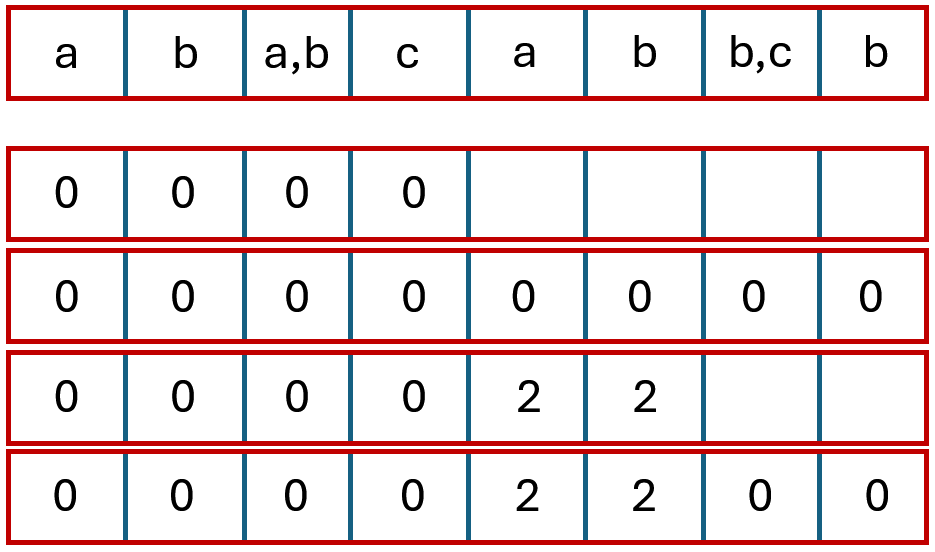
\includegraphics[width=12cm]{Images/backtrack_example.png}
\end{center}


\newpage

\subsubsection{Backtracking limitations}

Backtracking does yield viable and optimized solutions as it constantly checks for broken constraints
and can iterate through the whole search space (looking for the more valuable roll in our case). 
Although, our search space is huge for that kind of algorithms. There are 2,656,615,626 combinations of 500 elements 
(the roll integer positions) among 5 items ('None', '0', '1', '2', '3'). Formula given by:\\

\[ \Gamma^k_n=\binom{n+k-1}{k}=\frac{(n+k-1)!}{k!(n-1)!} \]\\

\subsubsection{Trying on a sample of the roll}

To test the backtracking algorithm on the biscuit problem, we reduced the roll's length to 50 units 
to compute a solution within our lifespan. We get a result after computing over 70,000,000 combinations:\\

\begin{figure}[h]
    \centering
    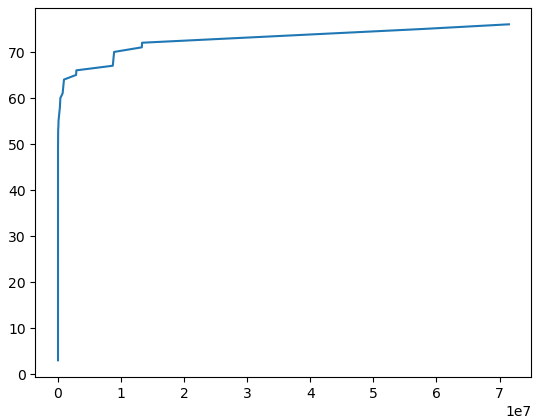
\includegraphics[width=12cm]{Images/ValuePlot_roll50.png}
    \caption{Best overall roll value per iteration. | Backtracking on a 50 units long roll.}
\end{figure}

\newpage

\subsection{Improving the solution : Parallelization}

Our algorithm works. But it's not optimized enough to give us solutions for greater roll length values in our lifespan. Let's try and optimize this.\\

Parallelizing tasks can help reduce global complexity. For instance:\\ there are 2,656,615,626 combinations (with repetition)
of 500 elements among 5 items. If we split the 500 items list into two 250 items list, we have 2 lists of 169,362,501 possible 
combinations of 250 elments among 5 items. Thus a total of 338,725,002 states to explore, a little more than a 86\% 
reduction in computation time.\\

if we further split our "main list", in for instance, 10 sub-lists of 50 elements. 
We are left with only 316,251 combinations of 50 elements among 5 items. 
Thus, a total of 3,162,510 states to explore, or an approximate 99,85\% reduction in computation time.\\

This technique would give us 10 optimized lists. We can suppose that the combination of 
these optimized sub-lists can yield a fair approximation of the best result in a more than reasonable amount of time.


\subsection{First result, note about complexity}


Parallelization gave us our first result. We managed to get a  \textbf{roll with a value of 758}. 
This roll is necessarily viable as the CSP eliminates any non-satisfying solution, in regard of the given constraints.\\

To compare later results, we also retrieved this solution's complexity. 
Complexity is a variable in our CSP that gets incremented by one in each loop the code enters. For instance, 
if our code calls a 'for i in range(100)' loop, the resulting complexity of our code is 100.\\

The complexity of the code that found this first solution is 139 283 905. 
When working with other algorithms, we'll focus on lowering this number while giving an answer close or better 
than the value of 758.\\

\newpage

\section{Neural Network and Genetic Algorithm}

\subsection{The Neural Network}

Another approach to solve complex problems can be Neural Networks. In a nutshell, Neural Networks take various values
as an input, process these values passing them through their nodes (neurons) to output another value. In our case,
we could imagine that for a given input, the Neural Network could give us the biscuit to place in a given tile.

\subsubsection{Our Neural Network's Architecture}

\textbf{First Architecture Idea}\\

To provide thoughtful results, our Neural Network needs to "see" enough information to give a correct guess regarding the
biscuit to place in a given tile. "Seeing" information means passing these informations as inputs. The information we want
to pass as input, regardless of the architure, would be the roll's defects. Then, the Neural Network would need to figure
out what biscuit to place depending on what defects he sees.\\

The question becomes, what defects to pass ? First, we may think that too many input might overflow the model with informations.
That's why the first architecture chosen took, for any random rank in the roll, the defects of the 20 following tiles. We could
then iterate this NN model along our roll incrementing the rank by the chosen biscuit's size. For instance, if it decided to
place a biscuit of size 4 at rank 0, we then make it run again at rank \[ 0+4=4 \] to ensure that we have no overlap.\\

\begin{figure}[H]
    \centering
    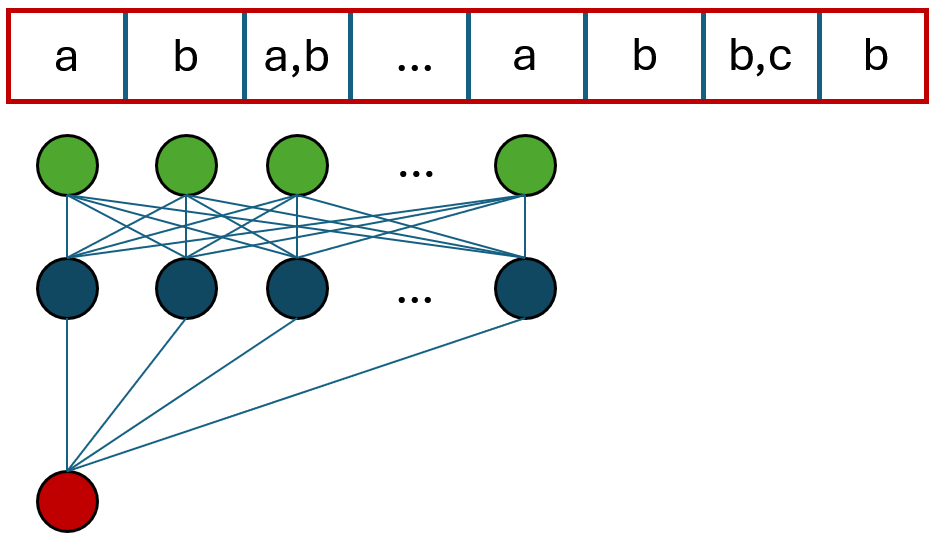
\includegraphics[width=10cm]{Images/NN_V1_A.png}
    \caption{First NN Architecture, Iteration n.}
\end{figure}

\begin{figure}[H]
    \centering
    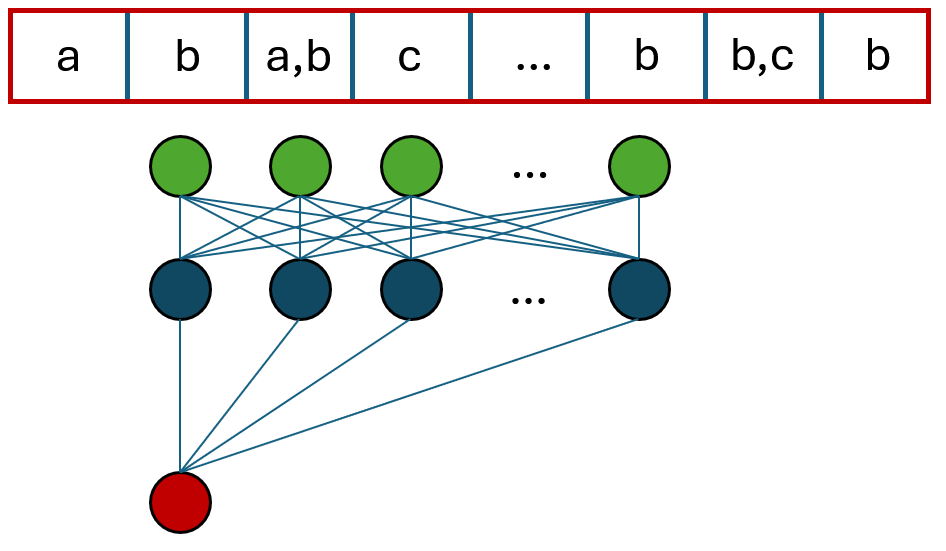
\includegraphics[width=10cm]{Images/NN_V1_B.png}
    \caption{First NN Architecture, Iteration n+1.}
\end{figure}

Even if this method worked, we wouldn't be able to go on after rank: \[roll_{size} - 20 \] as we'd lack defects informations 
to give our NN. Diminishing the size of the input would help but not come over this problem entirely. For instance,
reducing the number of input neurons to 10 would create a roll with the last 10 rank empty. We can get a good approximation
of the best roll but not the best yet. We can improve the architecture.

\textbf{Enhanced Architecture}\\

As we don't need 'real-time' computing speed (we're not controlling a robot), we can try to give the Neural Network the whole
roll's defects as input and ask it to yield the whole roll at once. The new architecture would look like the following:\\

\begin{figure}[H]
    \centering
    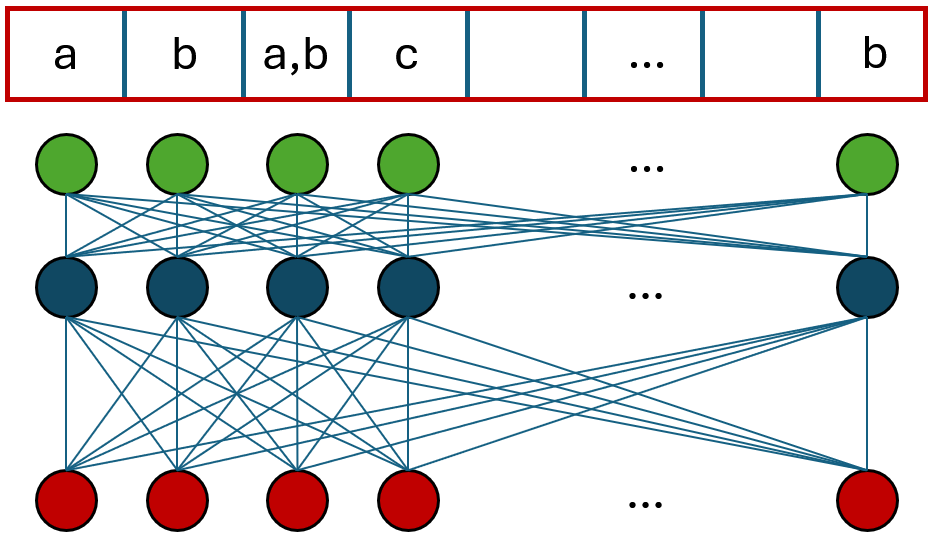
\includegraphics[width=12cm]{Images/NN_V2.png}
    \caption{Final NN Architecture}
\end{figure}

After some tweaking and empirical tests using the Genetic Algorithm defined in the following section, the Neural Network
ended up having only 1 hidden layer of 32 neurons to solve this problem. Each input neuron takes a tensor of 4 values as 
its input, formatted as [0. , 0. , 0. , 0.]. Each value of the tensor corresponds to the presence or not of a defect. For
instance, if we have defect a and b present, it would be [1. , 1. , 0. , 0.], the configuration [0. , 0. , 0. , 1.]
corresponds to no defect. The output neurons yield the probability of the tile belonging to each type. The tile gets 
assigned the value with highest probability. The domain of the values are [None, 0, 1, 2, 3]. So the output could be, for
instance, [0.93, 0.01, 0.02, 0.03, 0.01], in which case the corresponding tile would take the value "None".


\subsection{The Genetic Algorithm}

Now that our Neural Network and its architecture are defined, we must train it and make it yield good results. 

\subsubsection{What's a Genetic Algorithm ?}

A genetic algorithm is an optimization technique inspired by the principles of natural selection and genetics.
It operates by evolving a population of candidate solutions over several generations to solve a problem. 
Each candidate, is evaluated using a fitness function. The best-performing solutions are selected to produce 
offspring through operations like crossover and mutation. Over time, the population converges towards an optimal or 
near-optimal solution. Genetic algorithms are particularly effective for complex problems with large, 
nonlinear search spaces.

\subsubsection{Our population's evolution process}

To solve this problem using a genetic algorithm, we first initialize a population of potential solutions. Each individual 
in this population is a Neural Network with the architecture described precedently. What differentiates an individual form 
another is the weights inside of its neurons.\\

The first generation is initialized with random weight values, outputting random results regarding the biscuit placement 
along the roll. Every generation, all individuals are classified according to a fitness function. Our fitness function is 
the value of the roll, to which we substract penalties. Penalties are given when an individual gives a solution breaking 
constraints. The more constraints are broken, the more penalties we give.\\

Our Neural Network is built in such a way that it can't make biscuits overlap or get out of the roll's bounds. Thus, we 
can't break these two constraints and no penalty is applied there. The constraint we focus on is the biscuit's defects 
threshold. Every time a placed biscuit breaks a defects threshold, we remove 500 points to the fitness score of the 
individual. Punishing that roughly individuals breaking this constraint ensures the best individual of the last generation 
not to break it, and by extension, not break any of our constraint and give a viable solution, even if not optimal.\\

Top n individuals are considered as "elite" individuals and are taken to the next generation. Others go through tournament
selections (We pick the 2 best individuals of 4 randomly chosen). The ones who win tournament selection becomes parents of 
2 child, child made using two-points crossover. Childs are mutated and inserted into the next generation's population.\\

Note : Two-point crossover is a genetic algorithm operator used to combine the genetic information of two parent solutions to 
produce offspring. In this method, two crossover points are randomly selected within the parent individuals' informations. 
The segments between these points are swapped between the parents, creating two new offspring. This technique promotes 
diversity in the population while preserving some structure of the parent solutions.

\subsubsection{Preliminary results with Neural Network}

With the following settings:
\begin{itemize}
    \item Number of generations : 500
    \item Population size / generation : 100
    \item Number of elite individuals / generation : 10
    \item Mutation rate : 0.2
\end{itemize}

The best individual of the 500th generation yields a roll with a \textbf{value of 696}, for a complexity of 62,718,914.

\subsection{Parallelizing, again}

To further enhance the solution yielded by the genetic algorithm applied to our neural network, we can apply parallelization 
principles to this means of finding a solution to the problem. Thus, by dividing the 500 units long roll into 2 sub rolls of 250 units each, we can apply the genetic algorithm to 2 smaller 
neural networks, with 250 in/outputs rather than 500, greatly reducing computation time.\\

With the following settings on each sub-roll:
\begin{itemize}
    \item Number of generations : 200 (less generations needed as the problem gets 'easier' to solve by dividing it)
    \item Population size / generation : 100
    \item Number of elite individuals / generation : 10
    \item Mutation rate : 0.2\\
\end{itemize}

To make our best individual, we combine both best individuals of each sub-problem. The best individual 
yields a roll with a \textbf{value of 684}, for a complexity of 26,152,197.



\newpage

\section{Final results and comparison}

Overall here are our results :

\begin{table}[h]
    \centering
    \begin{tabular}{l|c|c|c|c}
        Algorithm & Value & $\Delta$Value (\%) & Complexity & $\Delta$Complexity (\%)\\ \hline
        CSP - Backtracking & N/A & $-$ & $+\infty$ & $-$\\ \hline
        CSP - Parallelized bckt & 758 & $-$\% & 149,283,905 & $-$\%\\ \hline
        NN - Genetic Algorithm & 696 & 8\% off & 62,718,914 & 58\% less\\ \hline
        NN - Parallelized GAs & 684 & 10\% off & 26,152,197 & 82\% less\\ \hline
    \end{tabular}

\end{table}

The final results highlight the performance of different algorithms in terms of solution value and computational complexity. 
The CSP Backtracking approach was unable to produce a valid solution due to its inability to handle the computational load, 
resulting in an infinite complexity. The CSP Parallelized Backtracking method significantly improved the feasibility, 
achieving a solution value of 758 but with high computational complexity. On the other hand, the Genetic Algorithm reduced 
the complexity by 58\%, achieving a value of 696, which is only 8\% off from the best found value. Finally, the Parallelized 
GA offered the best trade-off, reducing complexity by 82\% while maintaining a solution value of 684, just 10\% off the 
best value. This demonstrates the effectiveness of parallelization and evolutionary strategies in balancing performance and 
efficiency.\\

Side note : As biscuit 3 offers the best price/space ratio with a value of 1.6 per tile occupied, if we only had biscuit '3'
along the roll, not taking into account the defects thresholds the best theoretical value that the roll can have is 800.
Our best result, 758, is fairly close of this theoretical "no defects" best value, further justifying the usage of a CSP to
solve this problem.


\end{document}